% Third section

\section{Dynamic flying taxi scheduling}

The problem of dynamic flying-taxi scheduling consists in finding the optimal dispatching of a fleet of air taxis to serve a set of customers in real-time. In this context, some costumer requests as well as other problem parameters may not be known before the optimization starts. In the work of~\cite{panwadee2021}, a mixed-integer program was proposed to model this problem. Since this scheduling problem is NP-hard, exact methods may require long computation times to find an optimal solution. Thus, heuristic methods are more adapted to solve the real-time problem, where solutions must be computed in short times. For this reason, Panwadee~\cite{panwadee2021} used a genetic algorithm to solve the (static) problem.

In this section, we present two classical heuristics used in the field of the VRP to dispatch ground vehicles, namely the \acs{FCFS} and the \acs{NN}. The dynamic adaptation of these heuristics consists in integrating them in a rolling horizon approach. We will adapt these two heuristics to use them to solve the dynamic scheduling of flying taxis. The \acs{RH} approach we adopt is the \textit{periodic scheduling} strategy. The rolling domain in this context is a \textit{time-window}, \textit{i.e.}, a time slot on the scheduling horizon (see Figure~\ref{fig:rh}).

\begin{figure}[h!]
	\centering
	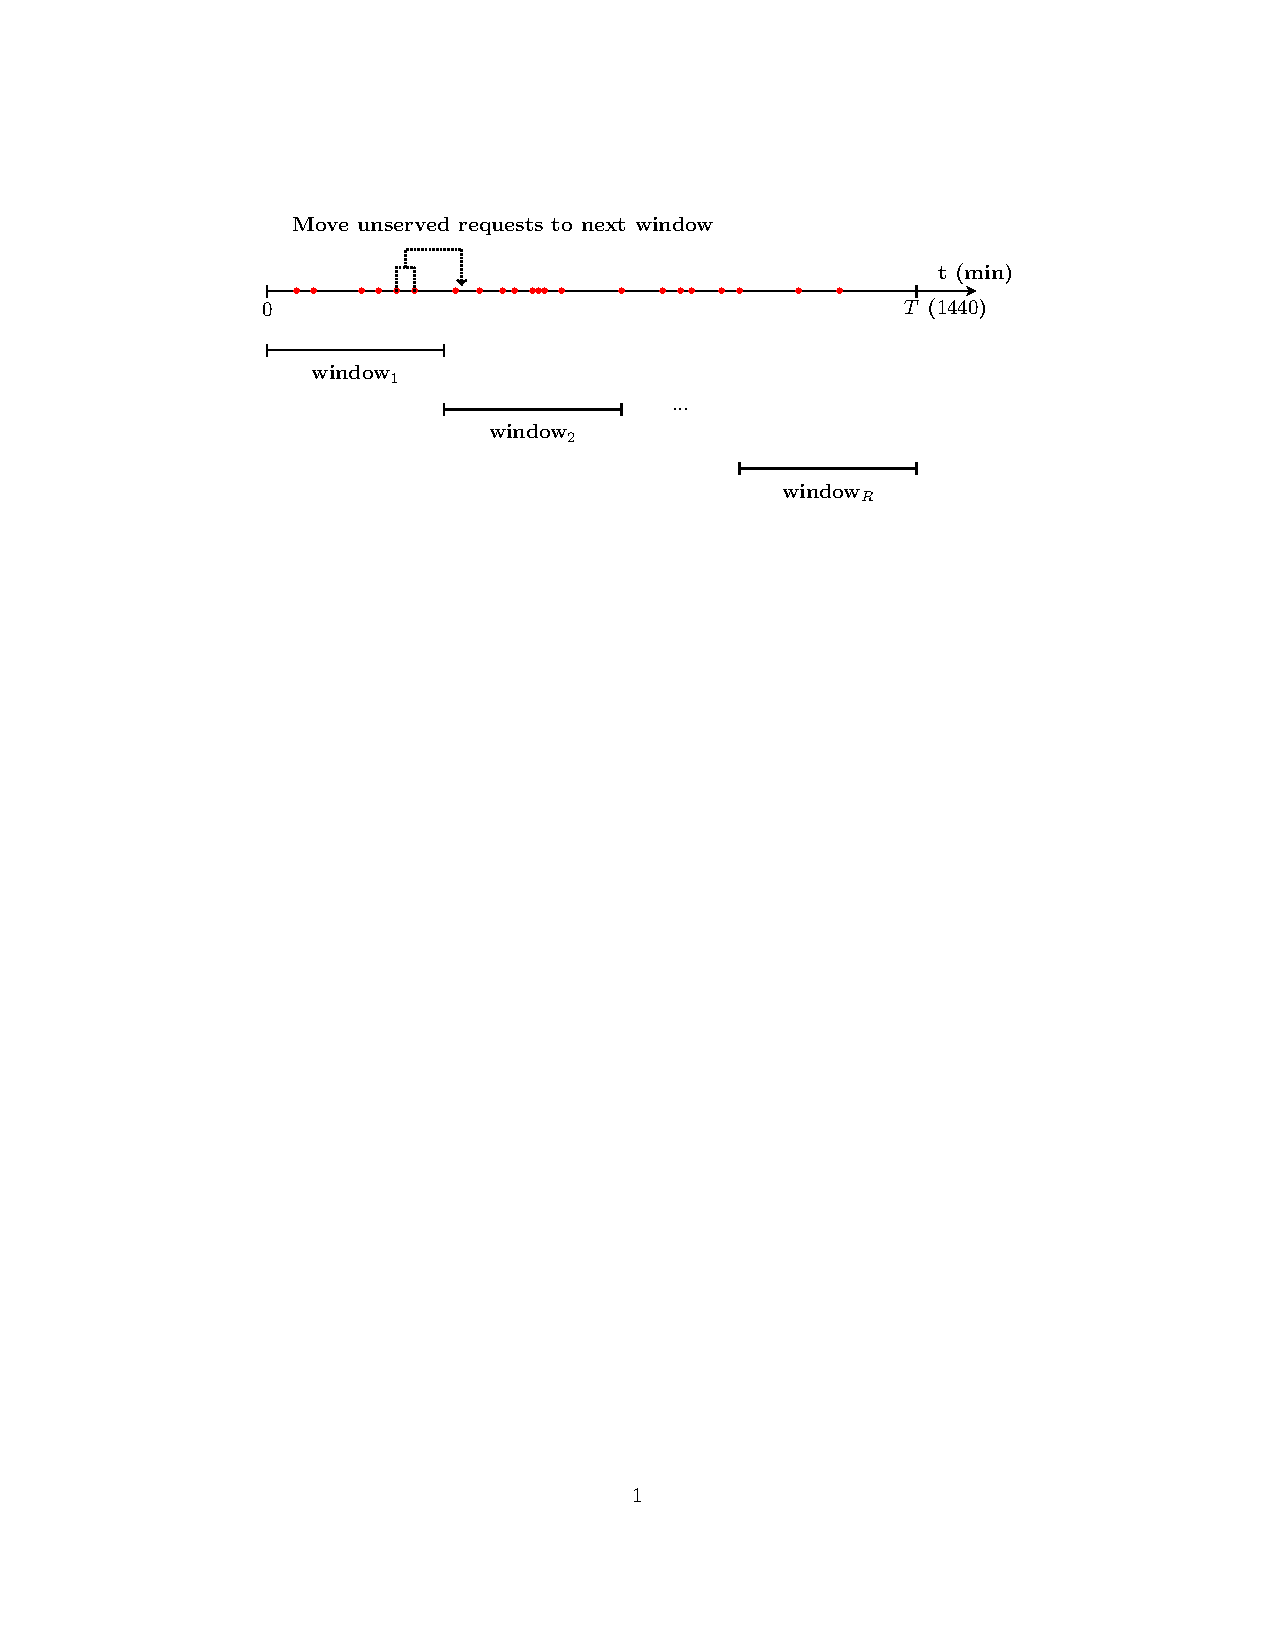
\includegraphics[trim=120 550 120 100,clip,width=0.85\textwidth]{images/rh-illustration.pdf}
	\caption{Rolling-horizon strategy with rolling time-windows.}
	\label{fig:rh}
\end{figure}

In the context of our \acs{RH} strategy, the (static) problem is solved in the first \textit{rolling window}, using a static scheduling heuristic (\acs{FCFS}, \acs{NN}, of the genetic algorithm of~\cite{panwadee2021}). At the end of this window, the \acs{RH} strategy moves the unserved requests to the beginning of the next window, and schedules them together with the new available requests in this window, as explained in Algorithm~\ref{alg:rh}.

\begin{algorithm}
	\caption{Rolling-horizon algorithm}\label{alg:rh}
	\begin{algorithmic}
		\Statex 1. \textbf{initialize} problem parameters (available taxis, battery level, scheduling horizon, rolling-window length)
		
		\Statex 2. \textbf{initialize} served and unserved requests ($=\emptyset$)
		
		\Statex 3. \textbf{for} each \texttt{rolling window} \textbf{do}
		
		\hspace{1cm} 4. \textbf{compute} available requests
		
		\hspace{1cm} 5. \textbf{append} non-served requests to available requests
		
		\hspace{1cm} 6. \textbf{apply a static scheduling heuristic} to schedule 
		
		\hspace{1cm} the available requests
		
		\hspace{1cm} 7. \textbf{update} served and non-served requests
		
		\hspace{1cm} 8. \textbf{update} battery level
		
	\end{algorithmic}
\end{algorithm}

The three scheduling heuristics that we use to solve the static problem inside each time window are explained in the next three sections.


\subsection{First-Come, First-Served}
\label{subsec:fcfs}

The \acs{FCFS} heuristic serves the requests according to the order given by their pick-up times. Indeed, the demands are sorted according to the non-decreasing order of their pick-up times. The advanced requests are served (without considering their locations) on their pick-up times or in an interval -- defined by the user -- centered around the pick-up time. The process continues until no request is available.

To illustrate how this heuristic works, let us consider an example. Suppose we have an instance with $2$ available flying taxis and $6$ requests, indexed by $1$, $2$, ..., $6$. The pick-up times (\texttt{pick\_t}) of each request is displayed in Table~\ref{tab:fcfs-exp}. The rows named \og\texttt{dur\_t}\fg, \og\texttt{ori\_x}\fg, \og\texttt{ori\_y}\fg, \og\texttt{des\_x}\fg, and \og\texttt{des\_y}\fg represent the duration, the x and y coordinates of the origin location of the request, and the x and y coordinates of the destination location, respectively.
\begin{table}
	\centering
	\begin{tabular}{ccccccc}
		\toprule
		\texttt{index}  &1     &  2    &    3  &    4  &    5   &   6\\
		\midrule
		\texttt{pick\_t}&   803 & 53    &  1373 &  1319 &  1425 &   710\\
		\texttt{dur\_t} &  26.1 & 19.17 &  30.01& 18.89 & 19.77 & 23.89\\
		\texttt{ori\_x} & 17182 &  5807 & 10958 & 12710 &  9890 & 10726\\
		\texttt{ori\_y} &  5391 &   828 & 21818 &  2405 & 21282 & 13201\\
		\texttt{des\_x} &  5753 & 10202 & 21534 & 20022 & 11893 & 21323\\
		\texttt{des\_y} & 12415 &  7076 &  8931 &  3602 & 13390 & 17863\\	
		\bottomrule
	\end{tabular}
	\caption{Example of an instance with $6$ requests.}
	\label{tab:fcfs-exp}
\end{table}

The \acs{FCFS} scheduler sorts the above-mentioned requests in the non-decreasing order of the pick-up times, then serves them in the resulting order. The battery level is checked before each customer pick-up, and updated after each customer drop-off. The solution provided by the \acs{FCFS} scheduler for our example is showed in Figure~\ref{fig:example-fcfs}. The green and orange bars illustrate the taxi service to serve the request and the battery recharging, respectively. 
\begin{figure}[h!]
	\centering
	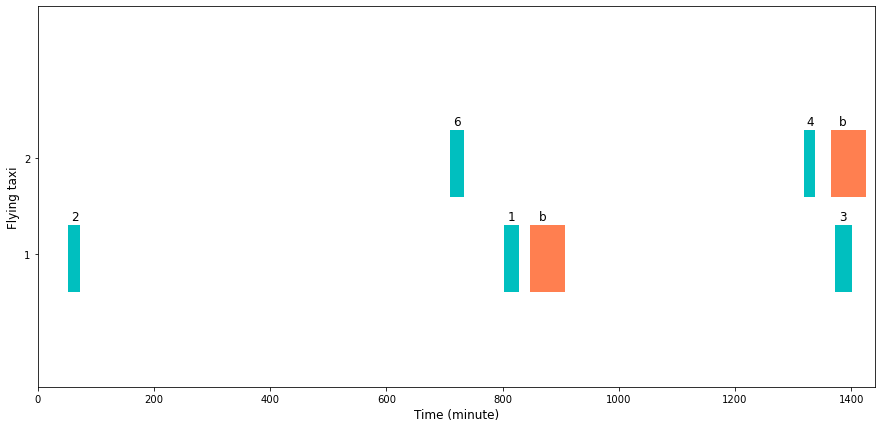
\includegraphics[width=0.9\textwidth]{images/example-fcfs}
	\caption{The \acs{FCFS} heuristic solution.}
	\label{fig:example-fcfs}
\end{figure}


\subsection{Nearest Neighbor}
\label{subsec:nn}

The \acs{NN} heuristic serves the closest requests to the current location of the taxi. Indeed, for each taxi, the \acs{NN} scheduler serves first the closest demand to the center. After completing service at the location of the first demand, the taxi travels to the nearest neighboring demand and so forth. The key difference between a \acs{FCFS} and a \acs{NN} scheduler is that the former sorts the customers at the beginning of the scheduling and then serves them, while the latter needs to compute the distances from current request location to all other unserved requests, to serve the closest one. This process is repeated after each customer drop-off to find the next one to serve. Hence, this heuristic may lead to larger computation times than the \acs{FCFS}.

If we consider the same example as in Section~\ref{subsec:fcfs}, the \acs{NN} heuristic solution is given in Figure~\ref{fig:example-nn}.

\begin{figure}[h!]
	\centering
	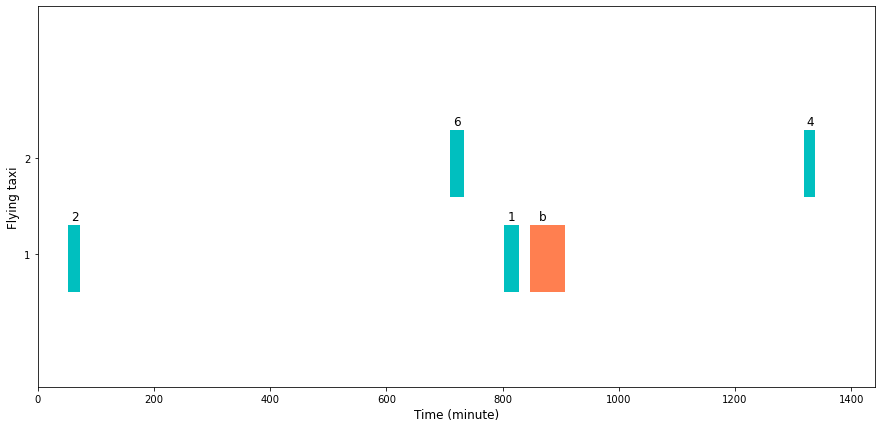
\includegraphics[width=0.9\textwidth]{images/example-nn}
	\caption{The \acs{NN} heuristic solution.}
	\label{fig:example-nn}
\end{figure}


\subsection{Genetic Algorithm}
\label{subsec:dynamic-ga}

The third heuristic that we integrate in the \acs{RH} approach is the \acs{GA} of~\cite{panwadee2021}, that was proposed to schedule flying taxis for the static case. In this \acs{GA}, the first population of chromosomes is randomly generated. Genetic operations such as mutations and crossovers are performed on this population, and best off-springs are selected to continue the process until the stopping criteria is satisfied. The latter corresponds to a number of iterations since the last improvement.

A chromosome is composed of genes whose values are randomly generated in the interval $[0,1]$.  Each gene represents a demand which is served by a flying taxi. Thus, the total number of genes in a chromosome is equal to the number of requests multiplied by the total number of taxis. For example, if we consider an instance with $3$ requests and $2$ flying taxis, the total number of genes is equal to $6$ (see Figure~\ref{fig:chromo})

\begin{figure}
	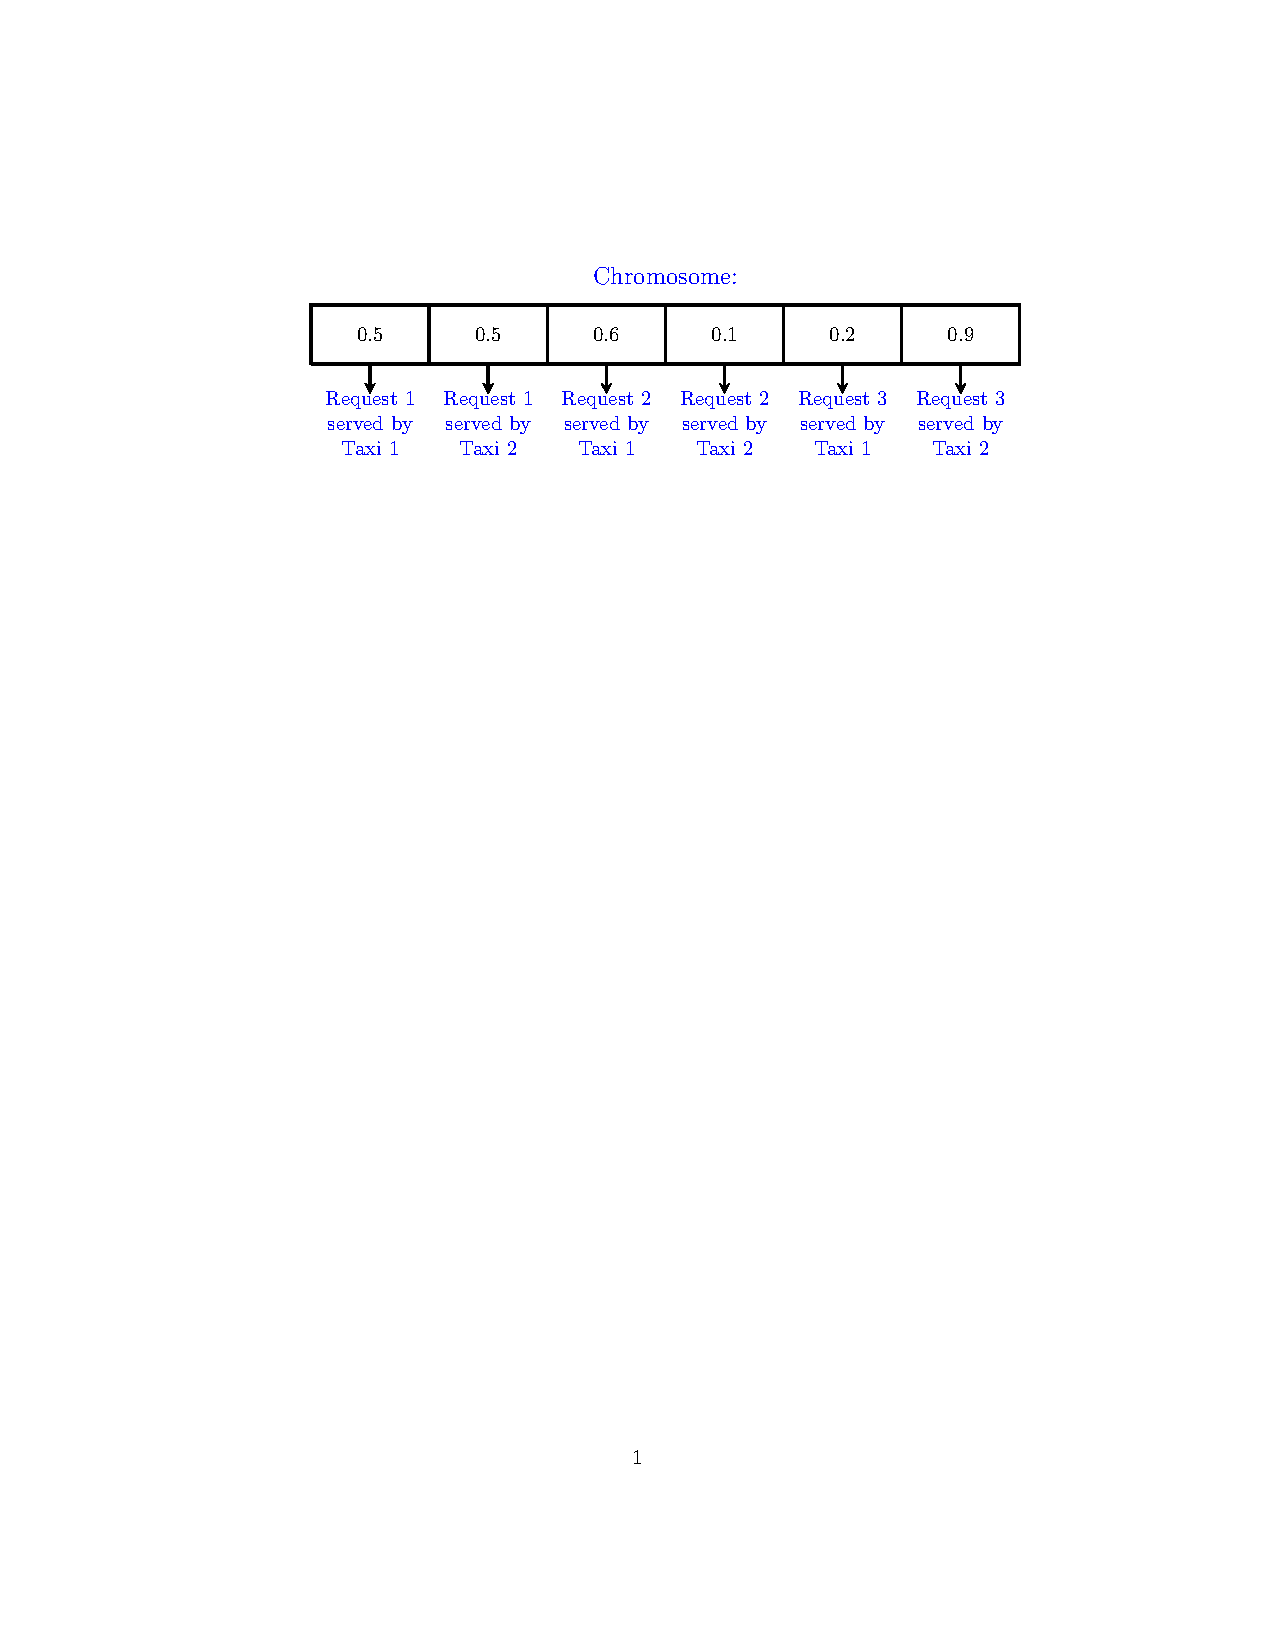
\includegraphics[trim=120 570 120 125,clip,width=0.85\textwidth]{images/chromosome.pdf}
	\caption{Example of a chromosome with six genes (3 requests/2 taxis).}
	\label{fig:chromo}
\end{figure}






